%%%%%%%%%%%%%%%%%%%%%%%%%%%%%%%%%%%%%%%%%%%%%%%%
% E.Pinault-Bigeard - e.pinault-bigeard@upsti.fr
% http://s2i.pinault-bigeard.com
% CC BY-NC-SA 2.0 FR - http://creativecommons.org/licenses/by-nc-sa/2.0/fr/
%%%%%%%%%%%%%%%%%%%%%%%%%%%%%%%%%%%%%%%%%%%%%%%%
\documentclass[11pt]{article}
%%%%%%%%%%%%%%%%%%%%%%%%%%%%%%%%%%%%%%%%%%%%%%%%
% Package UPSTI_Document
%%%%%%%%%%%%%%%%%%%%%%%%%%%%%%%%%%%%%%%%%%%%%%%%
\usepackage{subcaption}
\usepackage{UPSTI_Document}


\newcommandx*{\dessinRepereFigGeo}[5][1=\vx{},2=\vy{},3=\vz{},4=,5=0]
	{
		\draw [->,very thick] (0,0) -- (1,0) ;
		\draw [->,very thick] (0,0) -- (0,1) ;
    \fill[white] (0,0) circle (0.13);
    \draw [->,very thick] (0,0) circle (0.13);
    \ifnumequal{#5}{0} {% z vers nous
      \fill[black] (0,0) circle (0.03);
      \draw [->,thick] (0,0) circle (0.04);
    }{% z vers la feuille
  		\begin{scope} [rotate=45]
  			\draw [-,thick] (0,-0.12) -- (0,0.12) ;
  			\draw [-,thick] (-0.12,0) -- (0.12,0) ;
  		\end{scope}
    }
		\draw [anchor=north west] (1.1,0) node {${#1}$};
		\draw [anchor=south west] (0,1.1) node {${#2}$};
		\draw [anchor=north east] (-0.1,0) node {${#3}$};
		\draw [anchor=north west] (-0.1,-0.1) node {${#4}$};
	}

%---------------------------------%
% Paramètres du package
%---------------------------------%

% Version du document (pour la compilation)
% 1: Document prof
% 2: Document élève
% 3: Document à publier
\newcommand{\UPSTIidVersionDocument}{2}

% Variante
%\newcommand{\UPSTIvariante}{2}

% Classe
% 1: PTSI				6: PSI*			11: TSI2		16: Spé
% 2: PT	(par défaut)	7: MPSI			12: ATS
% 3: PT*				8: MP			13: PC
% 4: PCSI				9: MP*			14: PC*
% 5: PSI				10: TSI1		15: Sup
%\newcommand{\UPSTIidClasse}{2}

% Affichage personnalisé de la classe
\newcommand{\UPSTIclasse}{Première STI2D}

% Matière
% 1: S2I (par défaut)    2: IPT     3: TIPE
\newcommand{\UPSTIidMatiere}{5}

% Type de document
% 0: Custom*				7: Fiche Méthode			14: Document Réponses
% 1: Cours (par défaut)		8: Fiche Synthèse    		15: Programme de colle
% 2: TD     				9: Formulaire
% 3: TP						10: Memo
% 4: Colle					11: Dossier Technique
% 5: DS						12: Dossier Ressource
% 6: DM						13: Concours Blanc
% * Si on met la valeur 0, il faut décommenter la ligne suivante:
%\newcommand{\UPSTItypeDocument}{Custom}
\newcommand{\UPSTIidTypeDocument}{8}

% Titre dans l'en-tête
\newcommand{\UPSTItitreEnTete}{Programmation informatique}
%\newcommand{\UPSTItitreEnTetePages}{UPSTItitreEnTetePages}
%\newcommand{\UPSTIsousTitreEnTete}{UPSTIsousTitreEnTete}

% Titre
\newcommand{\UPSTItitrePreambule}{Arduino}
\newcommand{\UPSTItitre}{Bases de la programmation Arduino}

% Durée de l'activité (pour DS, DM et TP)
%\newcommand{\UPSTIduree}{3h}

% Note de bas de première page
%\newcommand{\UPSTInoteBasDePremierePage}{Note de bas de 1ère page}

% Numéro (ajoute " n°1" après DS ou DM)
%\newcommand{\UPSTInumero}{1}

% Numéro chapitre
\newcommand{\UPSTInumeroChapitre}{4}

% En-tête customisé
%\newcommand{\UPSTIenTetePrincipalCustom}{UPSTIenTetePrincipalCustom}

% Message sous le titre
%\newcommand{\UPSTImessage}{Message sous le titre}

% Référence au programme
%\newcommand{\UPSTIprogramme}{\EPBComp \EPBCompP{B1-02}, \EPBCompP{B2-49}, \EPBCompS{B2-50}, \EPBCompS{B2-51}, \EPBCompP{C1-07}, \EPBCompP{C1-08}}

% Si l'auteur n'est pas l'auteur par défaut
%\renewcommand{\UPSTIauteur}{UPSTI}

% Si le document est réalisé au nom de l'équipe
%\newcommand{\UPSTIdocumentCollegial}{1}

% Source
%\newcommand{\UPSTIsource}{UPSTI}

% Version du document
\newcommand{\UPSTInumeroVersion}{0.2}

%-----------------------------------------------
\UPSTIcompileVars		% "Compile" les variables
%%%%%%%%%%%%%%%%%%%%%%%%%%%%%%%%%%%%%%%%%%%%%%%%


%%%%%%%%%%%%%%%%%%%%%%%%%%%%%%%%%%%%%%%%%%%%%%%%
% Début du document
%%%%%%%%%%%%%%%%%%%%%%%%%%%%%%%%%%%%%%%%%%%%%%%%
\begin{document}
\UPSTIbuildPage

Nous avons vu plus tôt dans l'année, de la programmation graphique à l'aide du robot MoWay. Cette fiche synthèse s'intéresse à une approche textuelle de la programmation.

\UPSTIobjectif{	Durant cette séquence, vous avez réalisé un TP et une présentation portant notemment sur une carte Arduino. Cette fiche synthèse vous servira de support de cours et pour vos éventuels projets SIN de l'an prochain.

	Remplissez les différentes définitions avec vos propres mots.}

\tableofcontents


\section{Les composants principaux d'une carte Arduino}
\begin{figure}[h!t]
	\centering
	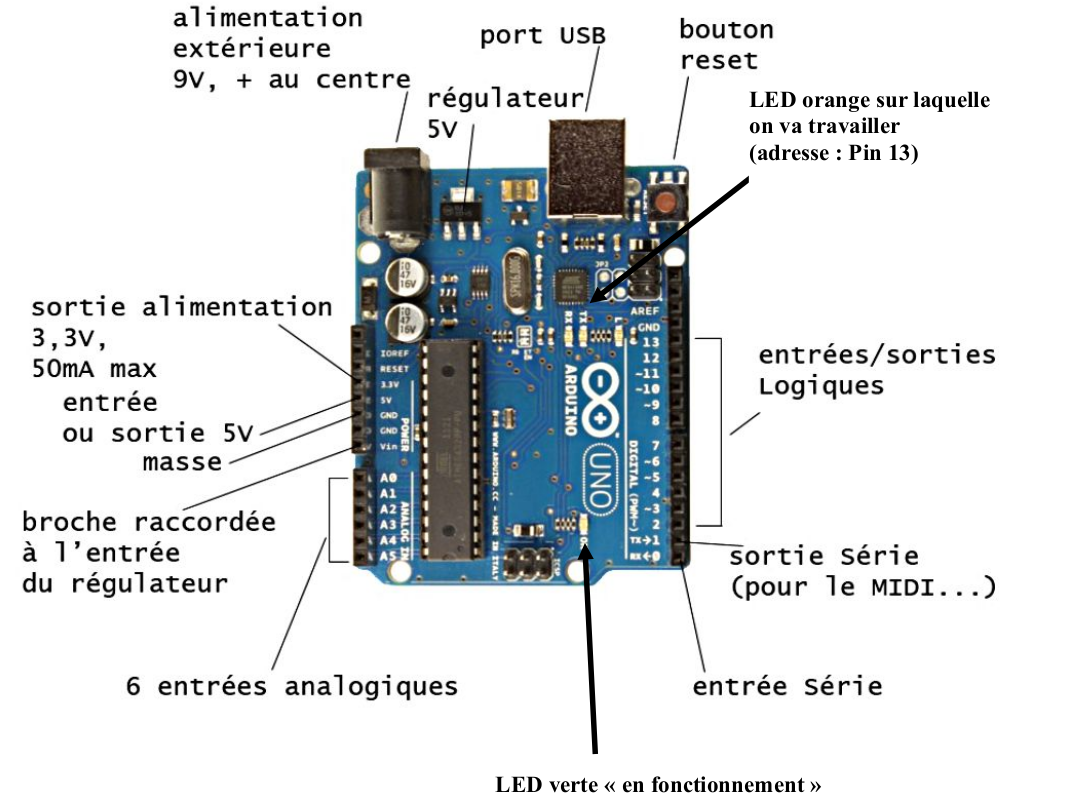
\includegraphics[height=.4\textheight]{Src/Images/arduino_schema}
	\caption{Schéma d'une carte Arduino}
	\label{fig:arduino_schema}
\end{figure}

Une carte \textit{Arduino} (illustrée en \UPSTIfig{fig:arduino_schema}) est une sorte de petit ordinateur. Il possède un microcontrôleur, composé d'un \textbf{microprocesseur}, d'une \textbf{mémoire} et d'une \textbf{interface de gestion des entrées/sorties.}


\UPSTIdefinition[Microprocesseur]{
\UPSTIeleveOnly{\UPSTIpointilles[2]}
\UPSTIprofOnly{\UPSTIaCompleter{Le microprocesseur est un « processeur miniature ». Il exécute les instructions et traite les données des programmes.}}
}

\UPSTIdefinition[Mémoire FLASH]{
\UPSTIeleveOnly{\UPSTIpointilles[2]}
\UPSTIprofOnly{\UPSTIaCompleter{Cette mémoire stoque les programmes à exécuter. C'est une mémoire qui perdure après arrêt de l'alimentation.}}
}

\UPSTIdefinition[Mémoire SRAM]{
\UPSTIeleveOnly{\UPSTIpointilles[2]}
\UPSTIprofOnly{\UPSTIaCompleter{Cette mémoire stoque les données temporaires (variables par exemple). Cette mémoire est volatile : elle est effacée lors de l'arrêt de la carte.}}
}

\UPSTIdefinition[Entrées/Sorties numériques]{
Une entrée/sortie est une connexion physique. Une "broche" sur laquelle on câble quelque chose (un voyant, un bouton, un capteur, \dots). Une entrée/sortie peut prendre trois états : \textit{HIGH}, \textit{LOW} ou \textit{INPUT}.

\begin{description}
	\item [HIGH : ]	\UPSTIeleveOnly{\dotfill \UPSTIpointilles[1]}%
	\UPSTIprofOnly{\UPSTIaCompleter{signifie que la broche génère un signal. Cet état se traduit généralement par une tension de 5 volts en sortie de la broche.}}
	\item [LOW : ]	\UPSTIeleveOnly{\dotfill \UPSTIpointilles[1]} \UPSTIprofOnly{\UPSTIaCompleter{signifie que la broche ne génère pas de signal. Cet état se traduit généralement par une tension de 0 volt en sortie de la broche.}}
	\item [INPUT : ]	\UPSTIeleveOnly{\dotfill \UPSTIpointilles[1]} \UPSTIprofOnly{\UPSTIaCompleter{Dans cet état, la broche ne génère aucun signal. L'état "haute impédance" signifie que la broche est "en lecture" (en entrée). C'est cet état qui permet de "lire" un bouton par exemple.}}
\end{description}}

\UPSTIpresenceProf{Faites vérifier cette page par le professeur.}
\pagebreak

\section{Structure d'un programme Arduino}
\begin{UPSTIactivite}
	A partir du dernier TP et en cherchant sur internet des ressources à propos de la \textbf{structure d'un programme arduino}, complétez cette section.
\end{UPSTIactivite}

\UPSTIcode{
				/* Zone de déclaration de ressources */\\\\
				/* Zone de déclaration de variables globales */\\
				int led = 13;\\
				int bp = 6;\\\\
				/* Fonction SETUP */\\
				void setup() {\\
				  // initialize the digital pin as an output.\\
				  pinMode(led, OUTPUT);\\
				  // initialize the digital pin as an input.\\
				  pinMode(bp, INPUT);\\
				}\\\\
				/* Fonction LOOP */\\
				void loop() {\\
				  // read digital input bp\\
				  int a = DigitalRead(bp);\\
				  if(a == 1){\\
				    digitalWrite(led, HIGH); // turn the LED on\\
				  }\\
				  else{\\
				    digitalWrite(led, LOW);  // turn the LED off\\
				  }\\
				}\\
}

\UPSTIaRetenir[Zone de déclaration des ressources]{
	\UPSTIpointilles
}

\UPSTIaRetenir[Zone de déclaration de variables globales]{
	\UPSTIpointilles
}

\UPSTIaRetenir[Fonction setup]{
	\UPSTIpointilles
}

\UPSTIaRetenir[Fonction loop]{
	\UPSTIpointilles
}

\UPSTIpresenceProf{Faites vérifier cette section par le professeur.}
\pagebreak
\section{Les variables}
\begin{UPSTIactivite}
	A partir du dernier TP et en cherchant des ressources sur internet, complétez cette section.
\end{UPSTIactivite}

\UPSTIaRetenir[En programmation à quoi sert une variable ?]{
	\UPSTIpointilles
}

\UPSTIaRetenir[Comment déclare-t-on une variable ?]{
	\UPSTIpointilles
}

\UPSTIdefinition[Les différents types de variables]{
	Les variables peuvent être de différents types :\\
	\vspace{.3em}
	\begin{description}
		\item [INT : ] \dotfill\\
		\vspace{.3em}
		\item [UNSIGNED INT : ] \dotfill\\
		\vspace{.3em}
		\item [LONG : ] \dotfill\\
		\vspace{.3em}
		\item [UNSIGNED LONG : ] \dotfill\\
		\vspace{.3em}
		\item [FLOAT : ] \dotfill\\
		\vspace{.3em}
		\item [DOUBLE : ] \dotfill\\
		\vspace{.3em}
		\item [STRING : ] \dotfill\\
		\vspace{.3em}
	\end{description}}

\pagebreak
\section{Les fonctions}

\UPSTIaRetenir[En programmation à quoi sert une fonction ?]{
	\UPSTIpointilles
}

\paragraph{De quoi est composé une fonction ?}
\UPSTIpointilles[8]


\end{document}
